% fig_alpha50_progression.tex
% Bar chart: alpha_50 progression across TR-11 -> TR-12 -> TR-13 -> TR-15
% Two groups: ag (phase-to-ground) and 3ph (three-phase)
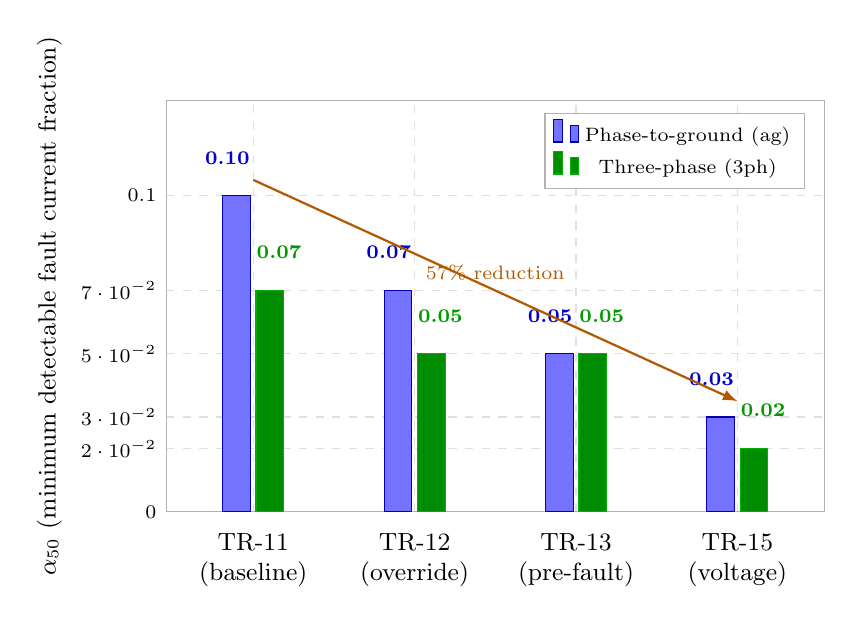
\begin{tikzpicture}
\begin{axis}[
  ybar,
  bar width       = 10pt,
  width           = 0.82\textwidth,
  height          = 6.8cm,
  enlarge x limits= 0.18,
  ylabel          = {$\alpha_{50}$ (minimum detectable fault current fraction)},
  ylabel style    = {font=\small},
  ymin = 0, ymax = 0.13,
  ytick           = {0, 0.02, 0.03, 0.05, 0.07, 0.10},
  yticklabel style= {font=\scriptsize},
  xtick           = {1, 2, 3, 4},
  xticklabels     = {
    {TR-11\\(baseline)},
    {TR-12\\(override)},
    {TR-13\\(pre-fault)},
    {TR-15\\(voltage)}
  },
  xticklabel style= {font=\small, align=center},
  legend style    = {at={(0.97,0.97)}, anchor=north east,
                     font=\scriptsize, draw=gray!60},
  legend columns  = 1,
  grid            = major,
  grid style      = {gray!25, dashed},
  tick style      = {draw=none},
  axis line style = {gray!60},
]

% ag fault bars (solid blue)
\addplot[fill=blue!55, draw=blue!70!black]
  coordinates {(1,0.10) (2,0.07) (3,0.05) (4,0.03)};
\addlegendentry{Phase-to-ground (ag)}

% 3ph fault bars (solid green)
\addplot[fill=green!55!black, draw=green!70!black]
  coordinates {(1,0.07) (2,0.05) (3,0.05) (4,0.02)};
\addlegendentry{Three-phase (3ph)}

% ---- Value annotations on bars -------------------------------------------
% ag values
\node[font=\scriptsize\bfseries, blue!80!black] at (axis cs:0.84, 0.112) {0.10};
\node[font=\scriptsize\bfseries, blue!80!black] at (axis cs:1.84, 0.082) {0.07};
\node[font=\scriptsize\bfseries, blue!80!black] at (axis cs:2.84, 0.062) {0.05};
\node[font=\scriptsize\bfseries, blue!80!black] at (axis cs:3.84, 0.042) {0.03};

% 3ph values
\node[font=\scriptsize\bfseries, green!60!black] at (axis cs:1.16, 0.082) {0.07};
\node[font=\scriptsize\bfseries, green!60!black] at (axis cs:2.16, 0.062) {0.05};
\node[font=\scriptsize\bfseries, green!60!black] at (axis cs:3.16, 0.062) {0.05};
\node[font=\scriptsize\bfseries, green!60!black] at (axis cs:4.16, 0.032) {0.02};

% ---- Improvement arrow ----------------------------------------------------
\draw[-latex, orange!70!black, thick]
  (axis cs:1.0, 0.105) -- node[above, font=\scriptsize, orange!70!black]
  {57\% reduction} (axis cs:4.0, 0.035);

\end{axis}
\end{tikzpicture}
